% Options for packages loaded elsewhere
\PassOptionsToPackage{unicode}{hyperref}
\PassOptionsToPackage{hyphens}{url}
%
\documentclass[
]{book}
\usepackage{amsmath,amssymb}
\usepackage{lmodern}
\usepackage{iftex}
\ifPDFTeX
  \usepackage[T1]{fontenc}
  \usepackage[utf8]{inputenc}
  \usepackage{textcomp} % provide euro and other symbols
\else % if luatex or xetex
  \usepackage{unicode-math}
  \defaultfontfeatures{Scale=MatchLowercase}
  \defaultfontfeatures[\rmfamily]{Ligatures=TeX,Scale=1}
\fi
% Use upquote if available, for straight quotes in verbatim environments
\IfFileExists{upquote.sty}{\usepackage{upquote}}{}
\IfFileExists{microtype.sty}{% use microtype if available
  \usepackage[]{microtype}
  \UseMicrotypeSet[protrusion]{basicmath} % disable protrusion for tt fonts
}{}
\makeatletter
\@ifundefined{KOMAClassName}{% if non-KOMA class
  \IfFileExists{parskip.sty}{%
    \usepackage{parskip}
  }{% else
    \setlength{\parindent}{0pt}
    \setlength{\parskip}{6pt plus 2pt minus 1pt}}
}{% if KOMA class
  \KOMAoptions{parskip=half}}
\makeatother
\usepackage{xcolor}
\IfFileExists{xurl.sty}{\usepackage{xurl}}{} % add URL line breaks if available
\IfFileExists{bookmark.sty}{\usepackage{bookmark}}{\usepackage{hyperref}}
\hypersetup{
  pdftitle={Reproducible Reporting: Cut Title Cost in Half},
  pdfauthor={Robert C. Cline, Sr., M.A., CPL},
  hidelinks,
  pdfcreator={LaTeX via pandoc}}
\urlstyle{same} % disable monospaced font for URLs
\usepackage{color}
\usepackage{fancyvrb}
\newcommand{\VerbBar}{|}
\newcommand{\VERB}{\Verb[commandchars=\\\{\}]}
\DefineVerbatimEnvironment{Highlighting}{Verbatim}{commandchars=\\\{\}}
% Add ',fontsize=\small' for more characters per line
\usepackage{framed}
\definecolor{shadecolor}{RGB}{248,248,248}
\newenvironment{Shaded}{\begin{snugshade}}{\end{snugshade}}
\newcommand{\AlertTok}[1]{\textcolor[rgb]{0.94,0.16,0.16}{#1}}
\newcommand{\AnnotationTok}[1]{\textcolor[rgb]{0.56,0.35,0.01}{\textbf{\textit{#1}}}}
\newcommand{\AttributeTok}[1]{\textcolor[rgb]{0.77,0.63,0.00}{#1}}
\newcommand{\BaseNTok}[1]{\textcolor[rgb]{0.00,0.00,0.81}{#1}}
\newcommand{\BuiltInTok}[1]{#1}
\newcommand{\CharTok}[1]{\textcolor[rgb]{0.31,0.60,0.02}{#1}}
\newcommand{\CommentTok}[1]{\textcolor[rgb]{0.56,0.35,0.01}{\textit{#1}}}
\newcommand{\CommentVarTok}[1]{\textcolor[rgb]{0.56,0.35,0.01}{\textbf{\textit{#1}}}}
\newcommand{\ConstantTok}[1]{\textcolor[rgb]{0.00,0.00,0.00}{#1}}
\newcommand{\ControlFlowTok}[1]{\textcolor[rgb]{0.13,0.29,0.53}{\textbf{#1}}}
\newcommand{\DataTypeTok}[1]{\textcolor[rgb]{0.13,0.29,0.53}{#1}}
\newcommand{\DecValTok}[1]{\textcolor[rgb]{0.00,0.00,0.81}{#1}}
\newcommand{\DocumentationTok}[1]{\textcolor[rgb]{0.56,0.35,0.01}{\textbf{\textit{#1}}}}
\newcommand{\ErrorTok}[1]{\textcolor[rgb]{0.64,0.00,0.00}{\textbf{#1}}}
\newcommand{\ExtensionTok}[1]{#1}
\newcommand{\FloatTok}[1]{\textcolor[rgb]{0.00,0.00,0.81}{#1}}
\newcommand{\FunctionTok}[1]{\textcolor[rgb]{0.00,0.00,0.00}{#1}}
\newcommand{\ImportTok}[1]{#1}
\newcommand{\InformationTok}[1]{\textcolor[rgb]{0.56,0.35,0.01}{\textbf{\textit{#1}}}}
\newcommand{\KeywordTok}[1]{\textcolor[rgb]{0.13,0.29,0.53}{\textbf{#1}}}
\newcommand{\NormalTok}[1]{#1}
\newcommand{\OperatorTok}[1]{\textcolor[rgb]{0.81,0.36,0.00}{\textbf{#1}}}
\newcommand{\OtherTok}[1]{\textcolor[rgb]{0.56,0.35,0.01}{#1}}
\newcommand{\PreprocessorTok}[1]{\textcolor[rgb]{0.56,0.35,0.01}{\textit{#1}}}
\newcommand{\RegionMarkerTok}[1]{#1}
\newcommand{\SpecialCharTok}[1]{\textcolor[rgb]{0.00,0.00,0.00}{#1}}
\newcommand{\SpecialStringTok}[1]{\textcolor[rgb]{0.31,0.60,0.02}{#1}}
\newcommand{\StringTok}[1]{\textcolor[rgb]{0.31,0.60,0.02}{#1}}
\newcommand{\VariableTok}[1]{\textcolor[rgb]{0.00,0.00,0.00}{#1}}
\newcommand{\VerbatimStringTok}[1]{\textcolor[rgb]{0.31,0.60,0.02}{#1}}
\newcommand{\WarningTok}[1]{\textcolor[rgb]{0.56,0.35,0.01}{\textbf{\textit{#1}}}}
\usepackage{longtable,booktabs,array}
\usepackage{calc} % for calculating minipage widths
% Correct order of tables after \paragraph or \subparagraph
\usepackage{etoolbox}
\makeatletter
\patchcmd\longtable{\par}{\if@noskipsec\mbox{}\fi\par}{}{}
\makeatother
% Allow footnotes in longtable head/foot
\IfFileExists{footnotehyper.sty}{\usepackage{footnotehyper}}{\usepackage{footnote}}
\makesavenoteenv{longtable}
\usepackage{graphicx}
\makeatletter
\def\maxwidth{\ifdim\Gin@nat@width>\linewidth\linewidth\else\Gin@nat@width\fi}
\def\maxheight{\ifdim\Gin@nat@height>\textheight\textheight\else\Gin@nat@height\fi}
\makeatother
% Scale images if necessary, so that they will not overflow the page
% margins by default, and it is still possible to overwrite the defaults
% using explicit options in \includegraphics[width, height, ...]{}
\setkeys{Gin}{width=\maxwidth,height=\maxheight,keepaspectratio}
% Set default figure placement to htbp
\makeatletter
\def\fps@figure{htbp}
\makeatother
\setlength{\emergencystretch}{3em} % prevent overfull lines
\providecommand{\tightlist}{%
  \setlength{\itemsep}{0pt}\setlength{\parskip}{0pt}}
\setcounter{secnumdepth}{5}
\usepackage{booktabs}
\ifLuaTeX
  \usepackage{selnolig}  % disable illegal ligatures
\fi
\usepackage[]{natbib}
\bibliographystyle{apalike}
\nocite{*}

\title{Reproducible Reporting: Cut Title Cost in Half}
\author{Robert C. Cline, Sr., M.A., CPL}
\date{2022-06-15}

\begin{document}
\maketitle

{
\setcounter{tocdepth}{1}
\tableofcontents
}
\hypertarget{introduction}{%
\chapter{Introduction}\label{introduction}}

The scientific community has invested heavily in what is known as reproducible research to make their work reproducible for themselves and for other scientists wishing to replicate their studies to verify findings or explore the subject further. Scientists do not deploy reproducible research for cost cutting, but to document their research, making it both reproducible and verifiable. The technology available to create reproducible research is not limited to the scientific communty. Any individual or organization can utitlize this technology to make one's own reporting reproducible. The advantages of reproducible reporting are many, including organizing resources, automating the presentation of data analysis, and compiling data into a report for publication or review. It is this automation of the process that saves as much as 50 percent of the time it takes to create land title reports. Reproduciblity turns the process into an iterative process, so, as the data changes, the reports themselves simply update automatically. Stated another way, much of our reporting and document preparation stays the same while only the data source changes. An example would be the preparation of oil and gas leases. Instead of a lease and offer letter being prepared for each Lessor, all packages can be prepared at once from one data source. The names, tracts, net minerals and bonus payments change for each lessor and for each project, only the data input changes. The process of producing multiple lease packages is one batch print operation. This is called parameterized reporting. The template remains the same. Only the data changes. A separate report is created for each Lessor, for example. The process is much more robust than ``mail merge'' operations. The reporing process actually recalculates results using the parameters for each report. Utilizing the computer to batch process leases, very little time is used in preparing the lease package documents. It reduces the process from time measured in hours or days into seconds. This is where reproducible reporting has a great advantage over traditional reporting methods both in savings of time and money. The time savings is huge.

\hypertarget{usage}{%
\section{Usage}\label{usage}}

While replication is a fundamental tenet of science, it is grossly under utilized in business applications; especially the title business. The process of preparing reports in the title industry is expensive and time consuming. The process of interpreting title ownership requires ``hands-on'' review of title documentation and a knowledge of land law, contract law, probate law, etc. However, the process of reporting the analysis can be shortened by utilizing the methodology of reproducible research. Reproducible reporting is a way of utilizing current technolgy to both create iterative types of reports known as parameterized reports, and as a way to organize the title ownership data into easily managed data which can be maintained in a centralized database and updated as necessary.

\hypertarget{about-the-author}{%
\section{About the Author}\label{about-the-author}}

I, Robert C. Cline, Sr., hold a Masters Degree in Clinical Psychology from University of Houston-Clear Lake and, I am an AAPL Certified Professional Landman. My family operated a sovereign title plant, \href{http://www.stxmaps.com/go/texas-historical-marker-wharton-county-abstract-company.html}{Wharton County Abstract Company} which was established by Attorney William S. ``Billie'' Brooks in 1890. My grandfather, Henry Augustus Cline, joined Billie Brooks in 1899. I started working in that plant at age 11, a barefooted boy copying documents in the court house, developing and printing the images for the abstractor to compile into Abstracts and Title Certificates. I worked in that plant throughout my high school years. After college, I attended a two year program at the University of Texas San Antonio Title School (UTSA), earning a certificate in the title insurance industry. I was a licensed closing officer in the title plant and was a certified Title Examiner for several title insurance underwriters including Chicago Title Insurance Agency and Minisota Title Insurance Company. A title examiner is a position that, by industry standards, requires a law degree and five years of practice of land title law. That requirement was waived because of experience and UTSA certification. I was a member of the Texas Land Title Association and was a Title Plant Examiner for that organization, examining the records of title plants for adequacy and accuracy of title plants which had applied for membership in the association.

In 1976, I joined the brokerage firm of I. Jon Brook, Jr.~as a petroleum landman. In 1980, went to work for Clayton Williams, Jr.~in the Austin Chalk as a landman. I have had many clients over the years working as an Independent landman, managing title research for clients, managing due diligence projects, leasing projects and seismic projects. I spent five years working for Brett Oil Company in Houston in due diligence acquisitions. I earned the master's degree while working full time in the oil and gas industry as a field landman. In 2010 to 2014, I managed the field operations for Fairways Exploration \& Production, LLC, acquiring 10,000 leases covering 400,000 acres. At that same time, I managed a 100 square mile seismic acquisition project for that company.

I also served as an expert witness in land titles for the famous Houston criminal attorney, \href{https://deguerin.com/}{Dick DeGguerin}.

Today, I am still employed as a landman operating a brokerage business \href{https://goldentriangleland.com/}{Golden Triangle Land Services, Inc.} out of Sidney, Nebraska with my partner, Coy Fisher. During the downturn in the industry in 2014 to 2020, I used the time to enhance my data literacy; I studied advanced statistics, learning methods to create reproducible research. I write R code, a statistical programming language with \href{https://www.rstudio.com/about/}{RStudio} and I write some python. I write in Excel VBA, Power Query, Power Pivot and I create MS Access applications utilizing knowledge of VBA. I use GIS in both R programming language and with QGIS, both of which are open source applications.

\hypertarget{about-this-document}{%
\section{About this document}\label{about-this-document}}

This proposal is written in the format of a book with the Bookdown package for R, and is made available online in the form of an HTML document, PDF format, and as eBook publication. I intend to maintain a live preview which will update as I edit and change the document on an as-needed basis.

\begin{Shaded}
\begin{Highlighting}[]
\NormalTok{bookdown}\SpecialCharTok{::}\FunctionTok{serve\_book}\NormalTok{()}
\end{Highlighting}
\end{Shaded}

\hypertarget{implications-for-reproducible-reporting}{%
\chapter{Implications for Reproducible Reporting}\label{implications-for-reproducible-reporting}}

In the world of scientific research, the purpose of data analysis is to make the data analysis as open and transparent as possible to be able to exactly reproduce any of the results that were produced by it \citep{andrewsChapterReproducibleData}.

The data analysis pipeline used by scientific researchers is analagous to the process of analyzing land title ownership. Title analysis begins with acquiring title information from public records, documenting the title chain, reading the title chain and interpreting the chain of ownership and reducing the ownership into numerical quantities. Mineral titles often have many owners with multiple classes of ownership, from royalty interests, production interests, mineral interests, term interests, life estate and remainder interests, severed or interests in both surface and mineral estates. These interests are commonly referred to the ``bundle of sticks,'' meaning, there are many classes of ownership in the mineral and surface estates. A title report analyzes these interests in the form of fractional ownership. Periods of ownership are important as well. In Nebraska, for example, an owner who has not documented a claim or had a transfer of interest in his severed mineral estate for a period of 23 years, is subject to claims of abandonment of the mineral interest by the surface owner. The individual owners interest must be compiled into an ownership report together with the contact information for each owner. Claims, such as \emph{Lis Pendens}, delinquent taxes, pending County and District Court suits must be documented when reporting the status of the title for each owner.

\hypertarget{the-hypothetical-title-report}{%
\section{The Hypothetical Title Report}\label{the-hypothetical-title-report}}

Ownership reports are commonly lengthy and contain a lot of data depending on the complexity of the title. Geographical areas where there is mineral production, the title can expected to be more complex and more time consuming to complete.

Creating title reports, like scientific research, is a multi-step process. The Gantt chart below outlines a hypothetical number of days that it could take for each step in the process of compiling ownerhship reports.

It is impossible, without reams of data, to provide cost estimates in dollar amounts that could be saved by using reproducible reporting. The cost of examining and reporting title ownership is just too varied to make any sense. However, time savings can be estimated by analyzing each step in the analyis as a percentage of time it takes to complete the process. In the example below, I estimate the time in days to create a hypothetical title report covering complex mineral title. The proportion of time spent on each step of the process will remain fairly constant and therefore, can be a reliable predictor in percentage of time/cost that can be saved. The more complex your title issues, the greater the savings.

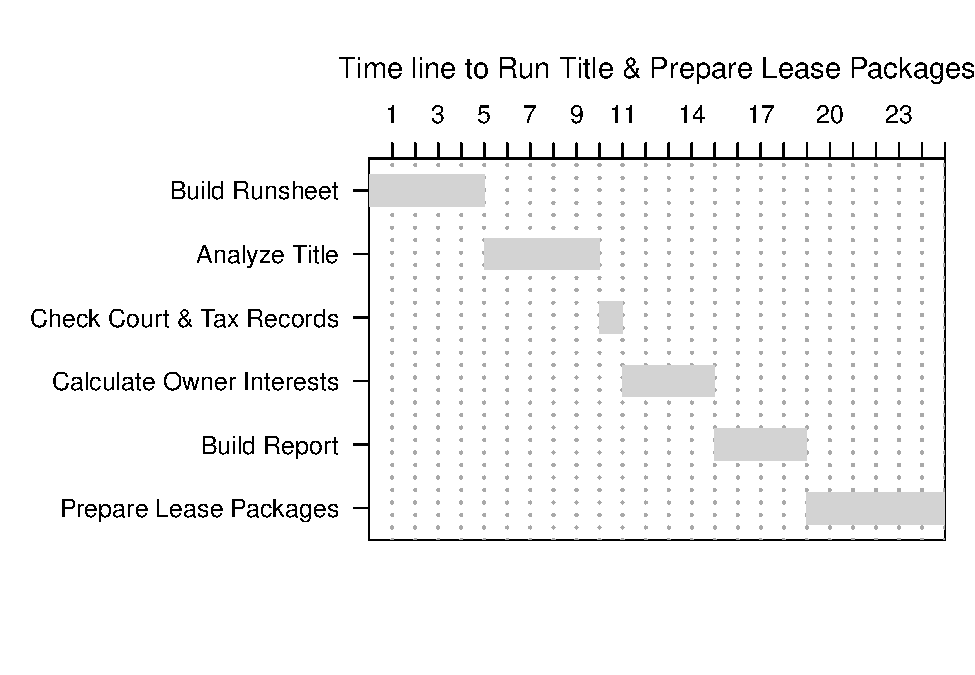
\includegraphics{01-intro_files/figure-latex/nice-fig-1.pdf}

The Gantt chart lists six steps for the preparation of an ownership report and preparation of lease packages. I have had some mineral titles that had as few as one owner and as many as 350 owners. Some titles may take a week or less to analyze, others may take a month or more. One never knows what title issues one will encounter, or how complex a title can be until one actually examines the title. The number of days chosen in the example below is simply a hypothetical case for illustration. What remain constant is, the time it takes to complete the first four steps is relative to the time it takes to complete steps 5 and six. That is, the number of days it takes to build the runsheet, analyize the title, and calculate the owners' interests, is equally proportional to the number of days it takes to build the report and prepare lease packages.

If, for example, one needs 15 days to get through calculating the owners' interests, one will need nearly that many days to build the report and prepare the lease packages. This is where reproducible reporting becomes an advantage.\\
Using the techniques of reproducible reporting, the time required for building the reports and preparing the lease packages is reduced from days to usually \emph{seconds}. It can actually cut the overall time involved in producing the reports in half. That time saved is a 50\% savings in labor cost.

This time saving advantage keeps on giving if changes to the report must be made. For example, if the report needs to be modified later, such as interest changing through sales or otherwise, only the data needs to be updated. The fractions are recalculated when the reports are generated. One does not have to re-write the ownership tables. If these are done in MS Word, for example, creating tables are a nightmare. Using R, the tables and fractional interests are automatically recalculated. If the report is published at a later date, those interests becoming subject to the abandonment statutes are also, automatically updated. Instead of re-writing a report, a simple change in the data for the report is made and the report is re-run automatically updating the calculations in seconds; or literally, fractions of a second.

\hypertarget{additional-benefits}{%
\subsection{Additional benefits}\label{additional-benefits}}

\href{https://us.sagepub.com/en-us/nam/author/mark-andrews}{Statistics professor Mark Andrews} \citep{andrewsChapterReproducibleData} emphasizes that reproducible data analysis is often motivated as a means of doing more high quality and robust data analyis and as a way of quality control that is essential to measure, identify errors, increase rigour and verify results and conclusions.\footnote{I took Mark Andrews' \emph{live} Online Course \emph{Reproducible Data Science Using RMarkdown, Git, R packages, Docker, Make \& Drake, and other tools} presented through PRStatistics.org on June 29 to July 4, 2020, \url{https://www.mjandrews.org/training/rdrp01/}} Mark Andrews offers as an example, a \$9bn loss of investment bank JPMorgan in 2012 \citep{ExcelMostDangerous2021}. Keeping data in Excel also has created vulnerabilities. In 2020, the Public Health England lost Covid data as a result of using Excel to collect data. One expert commented ``even a high-school computing student would know that better alternatives {[}to Excel{]} exist. \ldots{} you wouldn't use XLS, nobody would do that'' \citep{ExcelWhyUsing2020}.

\hypertarget{summary-of-savings-with-reproducible-reporting}{%
\subsection{Summary of Savings with Reproducible Reporting}\label{summary-of-savings-with-reproducible-reporting}}

Each title examination is different from any other, no two titles are the same. No title examiner ever knows what awaits. Predicting the length of time to complete the title examination and compile the reporting is not feasible. But, as a rule of thumb the process of reporting is relative to the complexity of title. The more complex the title, the longer the process of preparing reports and lease packages. With reproducible reporting, the time process is reduced from the time it takes to examine the title to almost zero. Thus, by employing reproducible reporting, the savings in terms of time spent, is rougly one-half. Reproducible reporting saves about 50\% of the time it normally takes to produce the same result.

\hypertarget{laying-the-groundwork-for-project-management}{%
\subsection{Laying the groundwork for project management}\label{laying-the-groundwork-for-project-management}}

Creating the infrastructure for reproducible reporting requires an understanding of the software used in reproducible reporting. R and its companion software, RStudio, are ideal for what is called parameterized reporting. Data literacy is becoming an important part of higher education. Landmen in today's world are taking on and accessing large amounts of data and some are even data mining. R does all this and it is open source which means it is free. Until land staff are educated in R basics, title persons do not need to process the output. People preparing the title reports will typically do so using templates prepared in CSV format. CSV files, or if prefered, XLSX files can be sufficient to acquire and process the data necessary for R to do its magic. The reporting can be created in commonly used media such as MS Word, PDF or HTML files.

Arguably, data is a company's most valuable asset. Without data, an organization becomes a foundering ship. Reproducible reporting is but one aspect of data literacy, but one in which title processes can be streamlined, time can be saved and costs can be reduced.

\begin{Shaded}
\begin{Highlighting}[]
\CommentTok{\#\textasciigrave{}r if (knitr::is\_html\_output()) \textquotesingle{}}
\CommentTok{\# References \{{-}\}}
\CommentTok{\#\textquotesingle{}\textasciigrave{}}
\end{Highlighting}
\end{Shaded}

\hypertarget{references}{%
\chapter*{References}\label{references}}
\addcontentsline{toc}{chapter}{References}

  \bibliography{book.bib,packages.bib}

\end{document}
